%% The comment character in TeX / LaTeX is the percent character.
%% The following chunk is called the header

\documentclass{article} % essential first line
\usepackage{times}    % this uses fonts which will look nice in PDF format
\usepackage{graphicx}   % needed for the figures
\usepackage{url}
\usepackage{adjustbox}
\usepackage{amsmath}
\usepackage{listings}
\usepackage{color}

\definecolor{dkgreen}{rgb}{0,0.6,0}
\definecolor{gray}{rgb}{0.5,0.5,0.5}
\definecolor{mauve}{rgb}{0.58,0,0.82}

\lstset{frame=tb,
  language=Java,
  aboveskip=3mm,
  belowskip=3mm,
  showstringspaces=false,
  columns=flexible,
  basicstyle={\small\ttfamily},
  numbers=none,
  numberstyle=\tiny\color{gray},
  keywordstyle=\color{blue},
  commentstyle=\color{dkgreen},
  stringstyle=\color{mauve},
  breaklines=true,
  breakatwhitespace=true,
  tabsize=3
}

%% Set the folder where pictures are located
\graphicspath{ {figures/} }

%% Here I adjust the margins

\oddsidemargin -0.25in    % Left margin is 1in + this value
\textwidth 6.75in   % Right margin is not set explicitly
\topmargin 0in      % Top margin is 1in + this value
\textheight 9in     % Bottom margin is not set explicitly
\columnsep 0.25in   % separation between columns

%% Define a macro for inserting postscript images
%% ==============================================
%% This is a macro which nominally takes 3 parameters, 
%% it would be used as follows to insert and encapsulated postscript
%% image at the location where it is used.
%%
%% \EPSFIG{epsfilename}{caption}{label}
%% - epsfilename is the name of the encapsulated postscript file to be
%%               inserted at this location
%% - caption is the text to be shown as the figure caption, it will be
%%           prepended by Figure X.  The number X can be referenced
%%           using the label parameter.
%% - label is a name given to the figure, it can be referenced using the
%%         \ref{label} command.

%\def\EPSFIG[#1]#2#3#4{   % Don't be scared by this monsrosity
%\begin{figure}[hbt]    % it is a macro to save typing later
%\begin{center}     % 
%\includegraphics[#1]{#2} %
%\end{center}     %
%\caption{#3}     %
%\label{#4}     %
%\end{figure}     %
%}        %

%% Define the fields to be displayed by a \maketitle command
\author{Timothy Dee, Brent Barth}
%{\it Undergraduate, Department of Electrical and Computer Engineering, Iowa State University}
%\author{Brent Barth}
%\it Undergraduate, Department of Electrical and Computer Engineering, Iowa State University}
\title{Lab 1 Report}

%%
%% Header now finished
%%

\begin{document}    % Critical
\twocolumn
\thispagestyle{empty}   % Inhibit the page number on this page
\maketitle      % Use the \author, \title and \date info

%% Next comes the abstract, notice the curly-braces surrounding the
%% text.

%%%%%%%%%%%%%%%%%%%%%
% PROJECT DESCRIPTION
%%%%%%%%%%%%%%%%%%%%%
%		CprE 458/558 Term Project Report Format (Sample)
%==========================================================================
%
%Here are some guidelines for the report. Page limits are mere suggestion,
%use number of pages as appropriate.
%
%There are three types of reports - survey, simulation, and implementation.
%
%Simulation/Implemenation Report Format (12-15 pages):
%
%       Project Summary  (1 page)
%       1. Introduction (2 pages)
%       2. Objectives and Scope (1 page)
%          Problem statement and Assumptions.
%       3. Solution Approach (3-4 pages)
%          3.1. Algorithm/Protocol (Discussion about the algo/protocol).
%          3.2 Illustrative Example
%       4. Simulation/Implementation (5 pages)
%          4.1. Simulation Model / Experimental Environment
%          4.2  Experiments and Analysis / Implementaion Details
%          4.3  Performance plots/ sample outputs / Sample screen output for GUI based simulator
%       5. Conclusions (3 pages)
%          5.1. Conclusion of the report; also, identify future work if relevant).
%          5.2  What did you learn by this project
%          5.3  Suggestion for such projects (feedback to the instructor)
%       References 
%%%%%%%%%%%%%%%%%%%%%%%%%%%%%%%%%%%%%%%%%%%%%%%%%%%%%%%%%%%%%%%%
% report should convey some sort of learning, beyond what we learned in class

\abstract{This report describes a gui simulation created for Cpre 458, Real Time Systems. 
The simulation depicts a car driving and the state of the processor on the car. 
The car is shown to be reacting to obstacles in accordance to the tasks being submitting.
The tasks are represented visually in a panel which depicts the state of the processor.
This paper also discusses the specific implementation of the program.}

% Insert description from original project proposal
\section{Project Summary}
%TODO

\section{Introduction}

%TODO

\section{Objectives and Scope}
%TODO

\section{Solution Approach}
\subsection{Algorithms}
%TODO

% give an example of our thing running i suppose?
\subsection{Solution Sample}
%TODO

\section{Simulation}
% block diagram of classes should probabally go here
\subsection{Simulation Model}
%TODO

\subsection{Implementation Details}
%TODO

% put a picture of the GUI screen here
\subsection{Outputs}
%TODO

\section{Conclusion}
\subsection{Synopsis}
%TODO

\subsection{Learning}
%TODO

\subsection{Suggestions}
%TODO


% listing example
\begin{lstlisting}[float=*,caption={Dynamic Frequency Scaling Mode II},label={lst:DFS_2},numbers=left]
hi
\end{lstlisting}

% figure example
\begin{figure}[!hbt]
\begin{center}
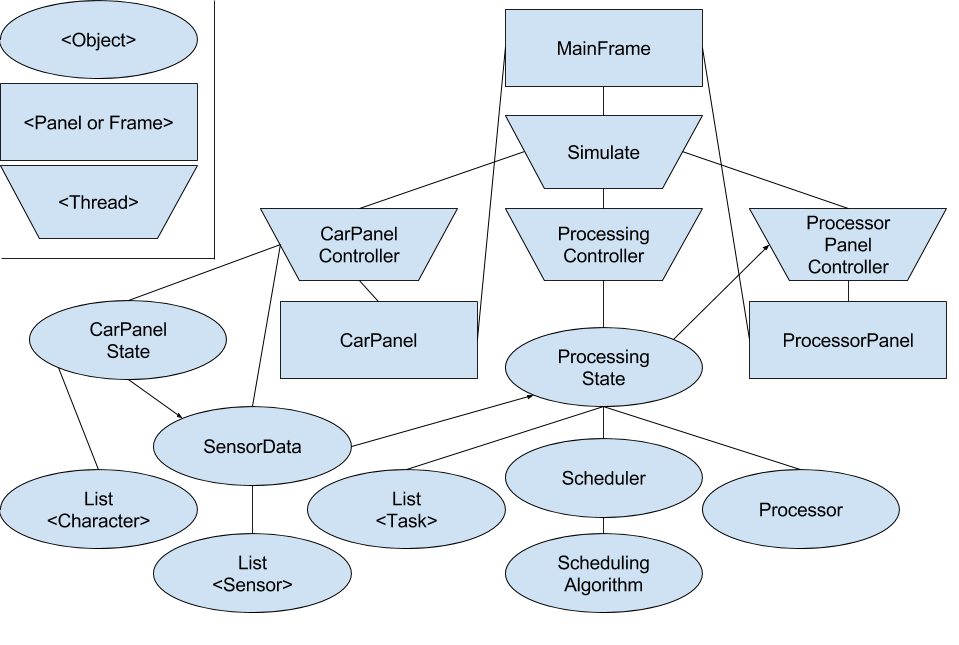
\includegraphics[width=.4\textwidth,keepaspectratio]{code_layout.png}
\end{center}
\caption{fig:Computation Time Vs Load}
\label{FIG-TRANSMITTER}
\end{figure}


%% This bit generates the references.  This part starts to get
%% slightly tricky.
\bibliographystyle{unsrt} % Order by citation
\bibliography{report}

\end{document}
